\documentclass[10pt]{beamer}
\usepackage[greek, english]{babel}
\usepackage{multirow}
\usepackage{fontspec}
\setsansfont{Arial}
\usepackage{unicode-math}
\usepackage{colortbl} 
\setmathfont{Latin Modern Math}
% \setsansfont{ebgaramond}
% Additional Font Packages (if desired)
%\usepackage{fontspec}
%\setmainfont{SomeFont}  % Use the font you prefer for text
\usetheme[
%%% option passed to the outer theme
%    progressstyle=fixedCircCnt,   % fixedCircCnt, movingCircCnt (moving is deault)
  ]{TUC}
  
% If you want to change the colors of the various elements in the theme, edit and uncomment the following lines
\definecolor{deepjunglegreen}{rgb}{0.0, 0.29, 0.29}
% Change the bar colors:
\setbeamercolor{TUC}{fg=deepjunglegreen!20,bg=deepjunglegreen}

% Change the color of the structural elements:
%\setbeamercolor{structure}{fg=red}

% Change the frame title text color:
%\setbeamercolor{frametitle}{fg=blue}

% Change the normal text color background:
%\setbeamercolor{normal text}{fg=black,bg=gray!10}

%-------------------------------------------------------
% INCLUDE PACKAGES
\usepackage[labelformat=empty]{caption}
\usepackage{media9}
\usepackage{animate}
\usepackage{hyperref}
\usepackage{xpatch}
\usepackage{pgfpages}
\usepackage{subfigure}
\usepackage{subcaption}
\usepackage{natbib}
\makeatletter
\xpretocmd\beamer@sectionintoc{\bigskip}{}{} % customize your skip here
\makeatother
%\setbeameroption{show notes on second screen}

%-------------------------------------------------------
%-------------------------------------------------------
% DEFFINING AND REDEFINING COMMANDS
%-------------------------------------------------------

% colored hyperlinks
\newcommand{\chref}[2]{
  \href{#1}{{\usebeamercolor[bg]{TUC}#2}}
}
\setbeamertemplate{itemize items}[circle]
%-------------------------------------------------------
% INFORMATION IN THE TITLE PAGE
%-------------------------------------------------------
\title[\textsf{3D Ανακατασκευή αντικειμένων με έμφαση στην κωδικοποίηση υψηλοσυχνοτικού περιεχομένου}]{\textsf{3D Ανακατασκευή Επιφανειών μέσω Έμμεσων Αναπαραστάσεων}}
\subtitle[]{\textsf{Έμφαση στην κωδικοποίηση υψηλοσυχνοτικού περιεχομένου}}

\author[Χάρης Φίλης]{\textsf{Χάρης Φίλης \hspace{0.1cm} AEM: 9449, \vspace{0.5cm} \\ Επιβλέποντες:\\ Αναστάσιος Ντελόπουλος, Καθηγητής\\  Αντώνης Καρακώττας, Υποψήφιος Διδάκτωρ \\ 
\hspace{9.2
cm} \tiny{Νοέμβριος, 2023}}}

\institute[School of Electrical \& Computer Engineering AUTH]
{       
      \vspace{3cm}
      SCHOOL OF ELECTRICAL \& \\
      COMPUTER ENGINEERING\\
      Aristotle University of Thessaloniki \\
  %there must be an empty line above this line - otherwise some unwanted space is added between the university and the country (I do not know why;( )
}


%-------------------------------------------------------
% THE BODY OF THE PRESENTATION
%-------------------------------------------------------

\begin{document}

%-------------------------------------------------------
% THE TITLEPAGE
%-------------------------------------------------------

{\1% % this is the name of the PDF file for the background
\begin{frame}[plain,noframenumbering] % the plain option removes the header from the title page, noframenumbering removes the numbering of this frame only
  \titlepage % call the title page information from above
\end{frame}}

\begin{frame}{Δομή Παρουσίασης}
    \begin{columns}[onlytextwidth,T]
        \begin{column}{.45\textwidth}
            \tableofcontents[sections=1-2]
        \end{column}
        \begin{column}{.45\textwidth}
            \tableofcontents[sections=3-4]
        \end{column}
    \end{columns}
\end{frame}

%-------------------------------------------------------
\section{Εισαγωγή}
\subsection{3D Ανακατασκευή}
%-------------------------------------------------------

\begin{frame}{Eισαγωγή}{Διατύπωση προβλήματος 3D ανακατασκευής}
    \note[item]{Η 3D ανακατασκευή αναφέρεται στις μεθόδους ανάκτησης της πληροφορίας του βάθους από μια αποτύπωση ή αποτυπώσεις του χώρου από πολλές όψεις το οποίο μπορεί να περιλαμβάνει και την φωτορεαλιστική απόδοση του πεδίου φωτισμού στον χώρο.}
\begin{itemize}
    \item Ανακατασκευή 3D μοντέλων από 2D εικόνες
    \begin{columns}
      \column{.4\textwidth}
      \begin{figure}
          \centering
            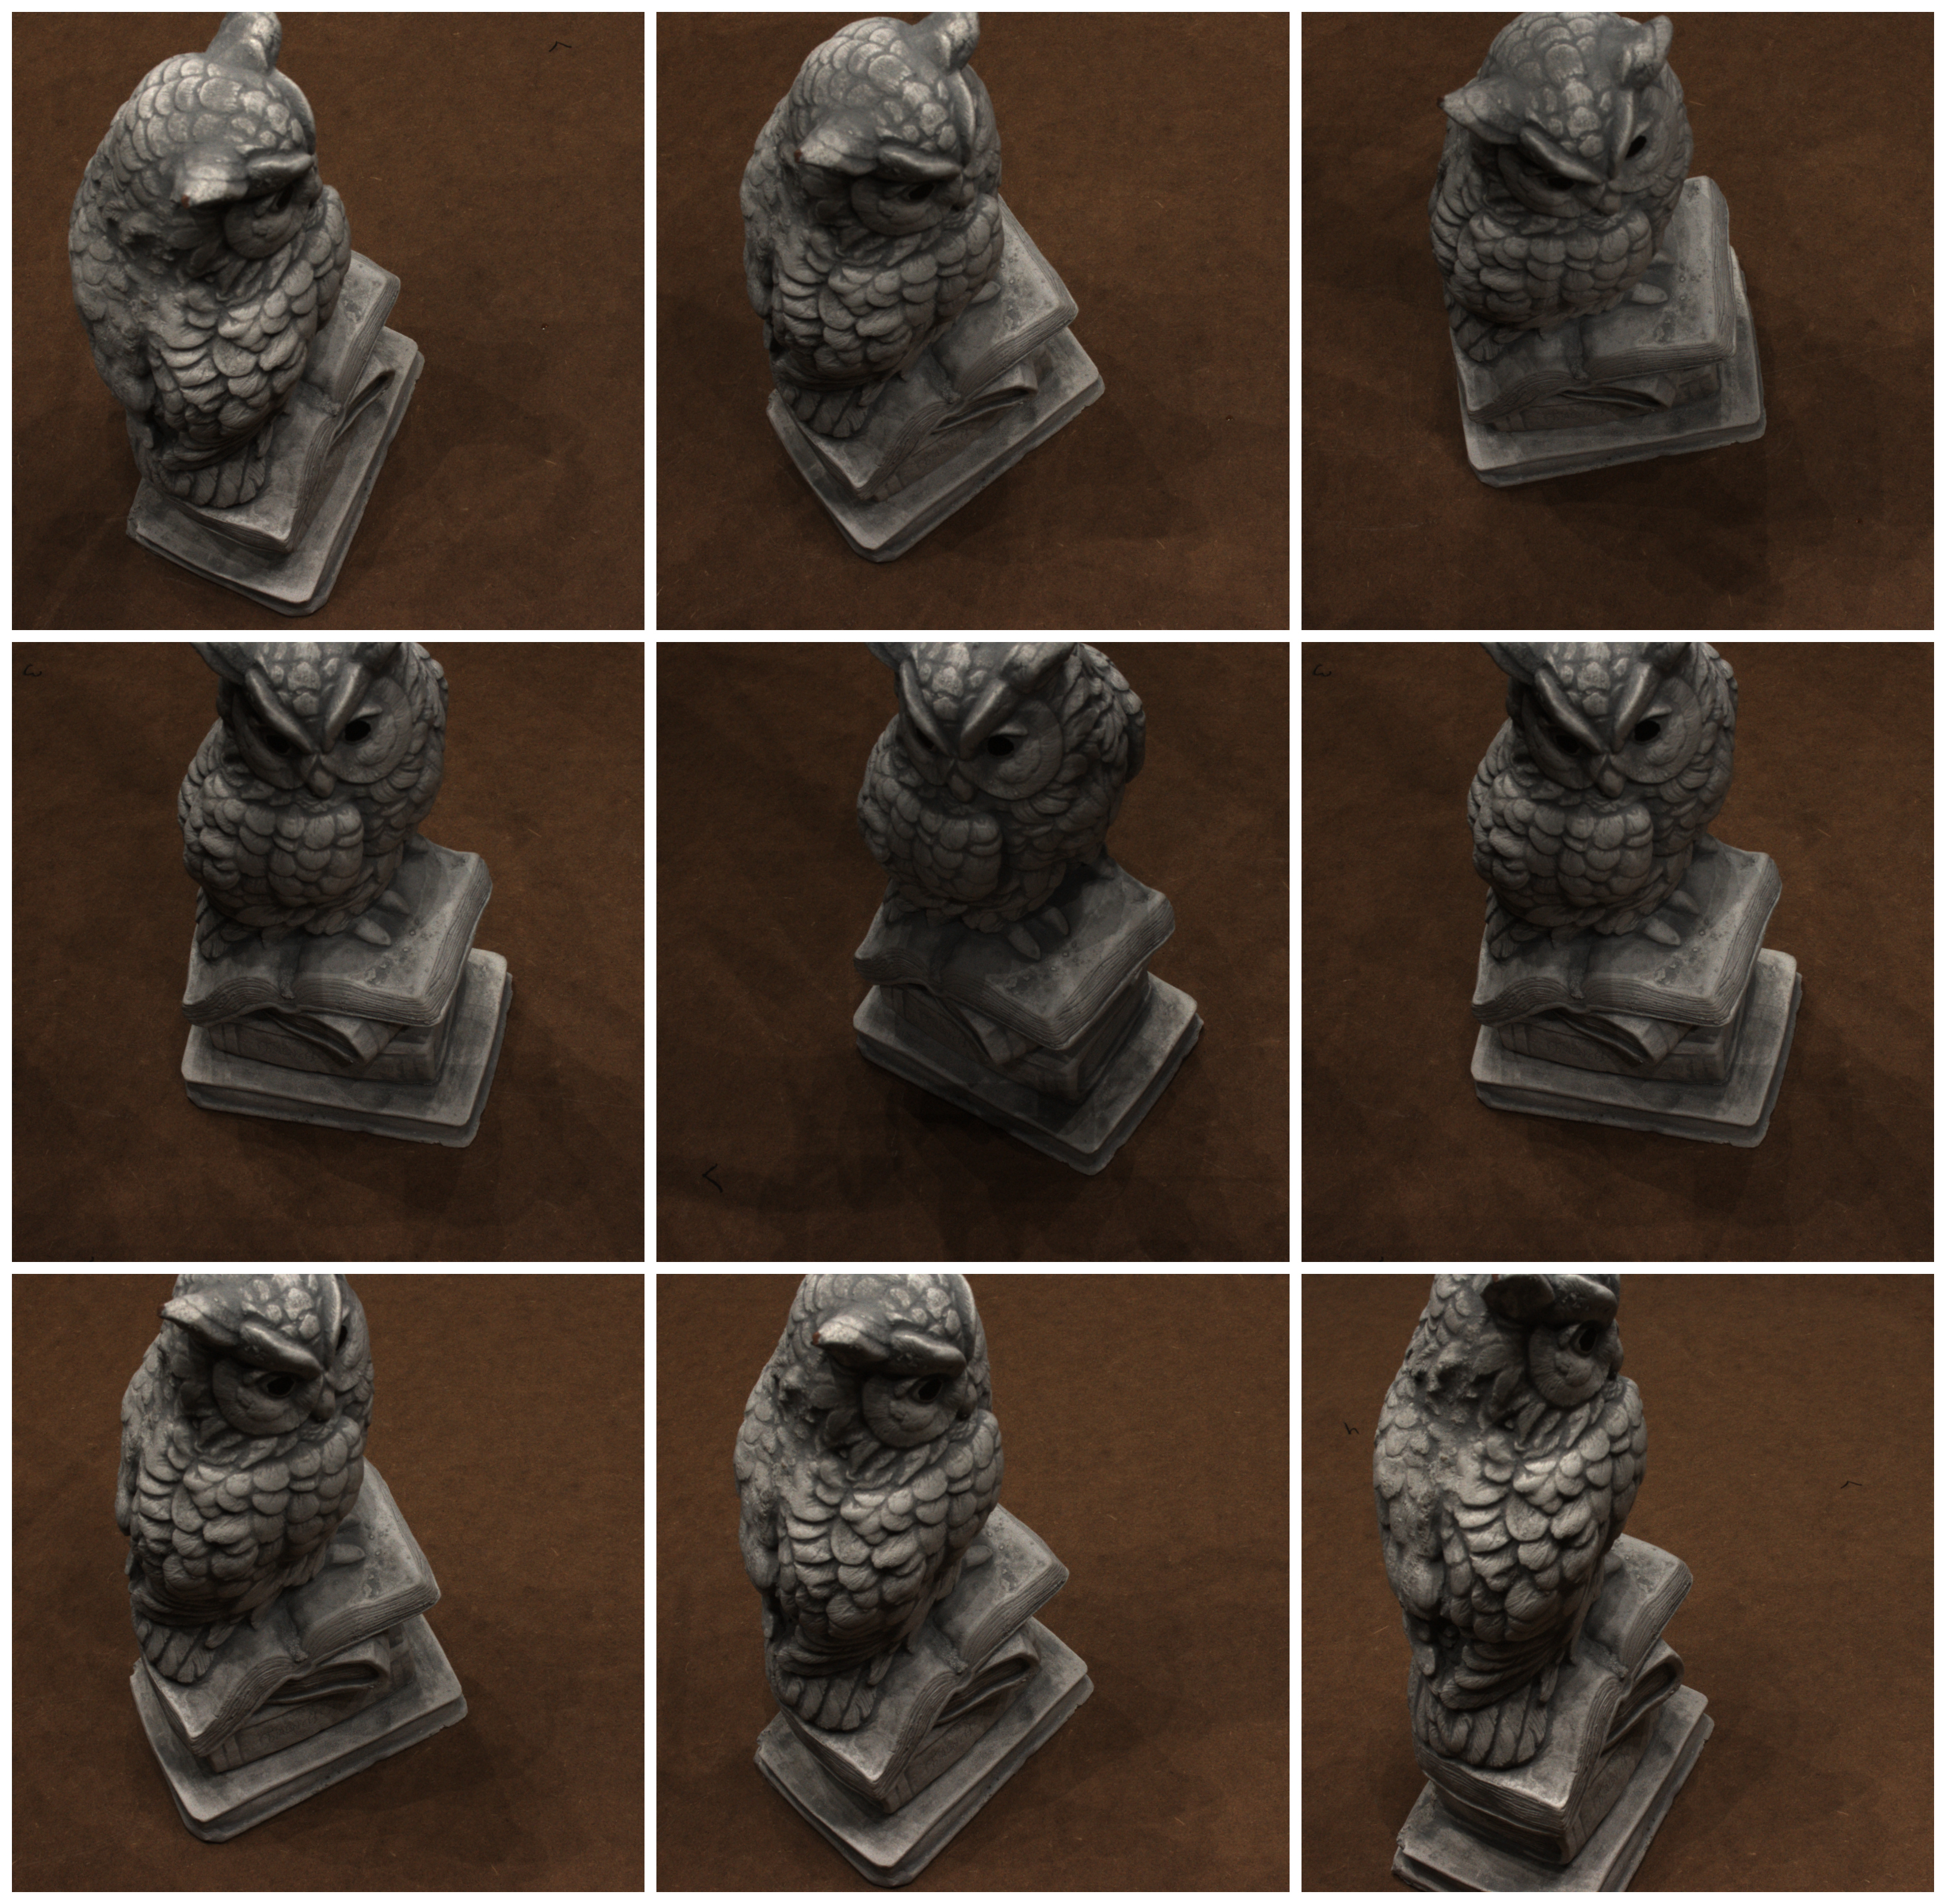
\includegraphics[height=.5\textheight]{images/122_Collage.jpg}
          {\caption*{Είσοδος συλλογή 2D εικόνων}}
          \label{fig:label}
      \end{figure}
      \column{.4 \textwidth}    
        \begin{figure}
            \animategraphics[loop,autoplay,width=5.5cm]{10}{./gifs/owl/owl-}{0}{14}
            \caption*{Έξοδος 3D Μοντέλο}
        \end{figure}
    \end{columns}
\end{itemize}
\end{frame}


\begin{frame}{Eισαγωγή}{Κίνητρο - Πεδία Εφαρμογής}
\begin{columns}
    
    \column{0.2\textwidth}
    \begin{figure}
        \centering
        \includegraphics[height=0.83\textwidth]{images/geodesic_field.jpg}
        \caption{Γεωδαισία}
        \label{fig:enter-label}
    \end{figure}\note[item]{Η 3D ανακατασκευή έχει πληθώρα }{}
    \column{0.2\textwidth}
    \begin{figure}
        \centering
        \includegraphics[height=0.7\textwidth]{images/3D_printed_implants.jpg}
        \caption{Ιατρική \\\small{3D εκτυπωμένα εμφυτεύματα, \\Εκμαγεία}}
    \end{figure}
    \column{0.2\textwidth}
    \begin{figure}
        \centering
        \includegraphics[height=0.83\textwidth]{images/Visualizing-a-two-dimensional-slice-of-the-signed-distance-field-SDF-PH-Blue-voxels.jpg}
        \caption{Ρομποτική \\ \small{ 3D Αντίληψη Χώρου}}
    \end{figure}
    \column{0.2\textwidth}
    \begin{figure}
        \centering
        \includegraphics[height=0.83\textwidth]{images/parthenon3drecon.jpg}
        \caption{Τέχνη, Ιστορία}
    \end{figure}
\end{columns}

\let\thefootnote\relax\footnote{\href{https://doi.org/10.1016/j.cageo.2011.09.012}{https://doi.org/10.1016/j.cageo.2011.09.012}}
\let\thefootnote\relax\footnote{\href{https://arxiv.org/abs/2204.02296}{https://arxiv.org/abs/2204.02296}}
\let\thefootnote\relax\footnote{\href{https://doi.org/10.1016/j.media.2008.12.003}{https://doi.org/10.1016/j.media.2008.12.003}}
\let\thefootnote\relax\footnote{\href{ https://doi.org/10.1111/cgf.12077}{ https://doi.org/10.1111/cgf.12077}}
\end{frame}
% \begin{frame}{Εισαγωγή}{Κλασσικές Μέθοδοι 3D Ανακατασκευής}
% \textbf{Γνωστή Θέση Καμερών}
% \begin{itemize}     
%     \item Ανάκτηση πληροφορίας βάθους μέσω πολλαπλών όψεων (Multi-View Stereo) με αντιστοίχηση χαρακτηριστικών (feature matching).
%     \item  NeRFs (Ben M. κ.α., 2020): Εκτίμηση ογκομετρικής πυκνότητας από ακτινοβολία που προέρχεται από ανεξάρτητες όψεις.
%     \item NeuS (P.Want κ.α., 2021) Εκτίμηση γεωμετρίας μέσω ογκομετρική αποτύπωσης
% \end{itemize}
%  \textbf{Άγνωστη Θέση Καμερών (χωρίς συμπαγή και πλήρη ανακατασκευή σκηνών)}  
% \begin{itemize}
%     \item Structure From Motion (SfM 2016)
%     \begin{enumerate}
%         \item Εκτίμηση από κοινού θέσης κάμερας και 3D αναπαράστασης 
%         \item Μειονέκτημα ότι λειτουργεί κυρίως σε αραιές αναπαραστάσεις (point cloud).
%     \end{enumerate}
%     \item COLMAP \let\thefootnote\relax\footnote{\href{https://colmap.github.io/}{https://colmap.github.io/}}
% \end{itemize}
    
% \end{frame}

\subsection{Αναπαραστάσεις Γραφικών}
\begin{frame}{Εισαγωγή}{Αναπαραστάσεις Γραφικών}
\begin{columns}
    \column{0.22\textwidth}
    \includegraphics[height = .5\textheight]{images/voxels.jpg} 
    \column{0.22\textwidth}
    \includegraphics[height = .5\textheight]{images/points.jpg} 
    \column{0.22\textwidth}
    \includegraphics[height = .5\textheight]{images/mesh.jpg}  \pause
    \column{0.22\textwidth} 
    \includegraphics[height = .5\textheight]{images/implicits.jpg} 
\end{columns}    
\end{frame}
\begin{frame}{Εισαγωγή}{Γιατί χρησιμοποιούνται Έμμεσες Αναπαραστάσεις;}
    \begin{columns}
        \column{0.65\textwidth}
        \begin{itemize}
            \item Μπορούν να αναπαρασταθούν(U.A.T.) ως ένα σύνολο εξόδου νευρωνικού δικτύου (Διαφορίσιμη Πολλαπλότητα - Νeural Level Set) 
            \item Αναπαριστούν  τον χώρο μέσω SDF\textbf{(Signed Distance Function)}
            \item H επιθυμητή επιφάνεια ανιστοιχεί στην Ισομετρική Επιφάνεια (Zero Level Set): \[S_{\theta} = \{\textbf{x} \in\mathbb{R}^{3}  |  f(\textbf{x};\theta) = 0\}\]
            \item Συντεταγμένες \((x,y,z) \in \mathbb{R}^{3} \rightarrow  \mathbb{R} \) (SDF Value)
            \item Δεν διακριτοποιούν το πρόβλημα της ανακατασκευής
            \item  Κωδικοποιούν την εμφάνιση του αντικειμένου 
        \end{itemize}
        \column{0.2 \textwidth}
        \begin{figure}
            \centering
            \includegraphics[height=0.6\textheight]{images/DeepSDFFields.jpg}
            \caption{SDF}
        \end{figure}
    \end{columns}
\end{frame}
\begin{frame}{Eισαγωγή}{Οπτική Απόδοση Αλγορίθμου Sphere Tracing σε πεδίο SDF}
    \begin{figure}
        \centering
        \includegraphics[width=\textwidth]{images/sphere_tracing3dviz.png}
    \end{figure}
\end{frame}
\section{Μεθοδολογία}
\subsection{Neural Implicit Rendering}
\begin{frame}[t]{Nευρωνική Αποτύπωση Έμμεσων Επιφανειών}{Neural Implicit Rendering - Ανάκληση/Inference}
    \begin{columns}[T]
    \centering
    \column{.4\textwidth}
    \includegraphics[height=.6\textheight]{images/NeuralRendering-Page-4.jpg} 
    \column{.5\textwidth}
        \textbf{Forward Pass:}
         \begin{itemize}
             \item \(\forall u \in {O(I)} \) 
             \item Sphere Tracing για εύρεση \(\hat{x}\) πάνω στην ακτίνα \(R_u(t) = \boldsymbol{c} + t \cdot\)v 
            \item Αν \(f_\theta \leq 0\) εντός , \(f_\theta \geq 0\) εκτός της επιφάνειας 
            \item Για \(\hat{x}\) (σημείο τομής) με εκτιμώμενη προσημασμένη απόσταση \( f( \hat{x})\) 
            \item Χρώμα Τexture Field \(\mathcal{M_\theta}(\hat{x})\) στο σημείο \(\hat{x}\)
            \item Εκτίμηση χρώματος pixel \(O(\hat{I_u})\) με αντίστροφή αποτύπωση
         \end{itemize}
        
    \end{columns}
\end{frame}
\begin{frame}[t]{Nευρωνική Αποτύπωση Έμμεσων Επιφανειών}{Neural Implicit Rendering - Oπισθοδιάδοση/Εκπαίδευση}
    \begin{columns}[T]
    \centering
    \column{.4\textwidth}
    \includegraphics[height=.6\textheight]{images/NeuralRendering-Page-3.jpg}     
    \column{.5\textwidth}
        \textbf{Backward Pass:}
         \begin{itemize}
             \item\(\mathcal{L}(\mathcal{O}(I),\mathcal{O}(\hat{I}))=\sum_{O_u}{|\hat{I}_u - \hat{I}|}\) \(\forall u \in {O(I)} \)
            \item Επιστροφή κλίσης σφαλμάτων στα βάρη των \(\mathcal{M},f\) δικτύων       \item Κανόνας Αλυσίδας
            \(\begin{aligned}
            \frac{\partial \mathcal{L}}{\partial \theta} & =\sum_{\mathcal{O}_\mathbf{u}} \frac{\partial \mathcal{L}}{\partial \hat{\mathbf{I}}_{\mathbf{u}}} \cdot \frac{\partial \hat{\mathbf{I}}_{\mathbf{u}}}{\partial \theta} \\
            \frac{\partial \hat{\mathbf{I}}_{\mathbf{u}}}{\partial \theta} & =\frac{\partial \mathbf{M}_\theta(\hat{\mathbf{x}})}{\partial \theta}+\frac{\partial \mathbf{M}_\theta(\hat{\mathbf{x}})}{\partial \hat{\mathbf{x}}} \cdot \frac{\partial \hat{\mathbf{x}}}{\partial \theta}
            \end{aligned}\)
            \item Έμμεση Διαφόριση σημείων τομής \(\hat{x}\) της εξίσωσης $f_\theta(\hat{x}(\theta,\tau);\theta)=0$, \fontsize{7}{7}\selectfont{ \(f_\theta(R_{u}(c + t(\theta,c(\tau),\)v\((\tau))*\)v\((\tau))\)\(;\theta)=0\) }
         \end{itemize}      
    \end{columns}
\end{frame}
\begin{frame}{Γενικό μοντέλο Rendering}{Light Field Approximation - P Universal Renderer}
\begin{columns}
  \column{.75\textwidth}
  \begin{block}{Πεδίο Ακτινοβολίας Επιφάνειας}
    \small{$$L(\hat{x},\boldsymbol{w^o}) = L^{e}(\hat{x},\boldsymbol{w^o}) +  \int_{\Omega}{B(\hat{x},\hat{n},\boldsymbol{w^i},\boldsymbol{w^o}) L^{i}(\hat{x},\boldsymbol{w^i})(\hat{n},\boldsymbol{w^i})dw^i}$$}
        \begin{itemize}
            \tiny{
            \item $L(\hat{x},\boldsymbol{w^o})$: Εκπέμπουσα ακτινοβολία από την σκηνή
            \item $B(\hat{x},\hat{n},\boldsymbol{w^i},\boldsymbol{w^o})$: Συνάρτηση κατανομής ανάκλασης διπλής κατεύθυνσης
            \item $L^{i}(\hat{x},\boldsymbol{w^i})$ Προσλαμβανόμενη ακτινοβολία στην επιφάνεια από άλλες πηγές φωτός
            \item $\hat{n}, \hat{w^i}$: κανονικά διανύσματα και διανύσματα εκπομπής (αποσβεστικοί παράγοντες στο μοντέλο κατοπτρικής ανάκλασης)
            \item $\Omega$: Σφαιρικό χωρίο επικεντρωμένο στο κανονικό διάνυσμα $\hat{n}$}
        \end{itemize}
    \end{block}
  \column{.3\textwidth}

      \includegraphics[height=.2\textheight]{images/BRDF_Diagram.jpg}

\end{columns}

\begin{block}{Restricted Lightfield - P Universality}
    Το συνεχές μέρος των P συναρτήσεων \(M_0\) περιγράφεται από ένα επαρκώς βαθύ MLP δίκτυο
    \[L(\theta,\gamma\ ,\tau) = M(\hat{x},\hat{n},\boldsymbol{v};\gamma)\]    
\end{block} 
\end{frame}
\subsection{IDR}


\begin{frame}{Mεθοδολογία}{Αρχιτεκτονική Δικτύου IDR}
\begin{figure}
    \centering
    \includegraphics[width=\textwidth]{images/idr-network-architecture.png}
\end{figure}

\end{frame}
\begin{frame}{Μεθοδολογία}{Συναρτήσεις Κόστους - Loss Functions}
    \begin{block}{Συνολική Συνάρτηση Κόστους}
    $$
    \operatorname{loss}(\theta, \gamma, \tau) = \operatorname{loss}_{\mathrm{RGB}}(\theta, \gamma, \tau) + \rho \operatorname{loss}_{\mathrm{MASK}}(\theta, \tau) + \lambda \operatorname{loss}_{\mathrm{E}}(\theta) $$
\end{block}
    
\end{frame}
\begin{frame}{Μεθοδολογία}{Συναρτήσεις Κόστους - Loss Functions}
\begin{block}{Φωτομετρικό Σφάλμα RGB (Εμφάνιση)}
    \[\mathrm{Loss}_{\mathrm{RGB}}(\theta,\gamma,\tau)=\frac{1}{|P|}\sum_{u\in P^{\mathrm{in}}}|I_{u}-L_{u}(\theta,\gamma,\tau)|\]
\end{block}
\begin{block}{Cross Entropy - Σφάλμα Μάσκας (Γεωμετρία)}
        \[\mathrm{Loss}_{\text{MASK}}(\theta,\tau)=\frac{1}{\alpha|P|}\sum_{u\in P^{\text{out}}}\mathrm{CE}(\mathcal{O}_u,\mathcal{S}_{u,\alpha}(\theta,\tau)) \]
\end{block}
\begin{block}{Παράγοντας Κανονικοποίησης Σημείων - Σφάλμα Εικονικής Εξίσωσης (SDF)}
    \[{{\mathrm{Loss}_{\mathrm{Eikonal}}(\theta)=\mathbb{E}_{x}{\Big(}\Vert\nabla_{x}f(x;\theta)\Vert-1\Big)^{2}}}\]
\end{block}
\end{frame}


\begin{frame}{Χρήση Υψηλοσυχνοτικής Κωδικοποίησης}{Ποιο είναι το πρόβλημα σε αυτή την αρχιτεκτονική;}
        \begin{block}{Προβλήματα Coordinate based MLP}
            \begin{itemize}
            \item Τα δίκτυα συντεταγμένων \(F(x,y,z;\theta)\) είναι \textbf{MLP} δίκτυα με \textbf{ReLU,SoftPlus} συναρτήσεις ενεργοποίησης ή γενικότερα τμηματικά γραμμικές συναρτήσεις που δεν έχουν την ικανότητα (\textbf{capacity}) να αποτυπώσουν υψηλοσυχνοτικές λεπτομέρειες της εικόνας στην έμμεσα αναπαριστώμενη επιφάνεια.
            \item Δεν λαμβάνονται υπόψιν σχέσεις που υπάρχουν σε υψηλότερες  διαστάσεις μεταξύ των δεδομένων.
            \end{itemize}
        \end{block} \pause
        \begin{alertblock}{Εκπαίδευση}
             Το πρόβλημα έχει τις ρίζες του και στην ίδια την δομή των νευρωνικών δικτύων και την διαδικασία της εκπαίδευσης
        \end{alertblock}\pause
        \begin{exampleblock}{Προτεινόμενη λύση} 
            Κωδικοποίηση-Μετασχηματισμός Εισόδου(\textbf{Input Εmbedding})
        \end{exampleblock}
        
\end{frame}
\begin{frame}{Χρήση Υψηλοσυχνοτικής Κωδικοποίησης}{Neural Frequency Input Embedding}
    \begin{figure}
        \centering
        \includegraphics[height=.4\textheight,width=\textwidth]{images/IDRwithEncoding.jpg}
    \end{figure}
\end{frame}

\begin{frame}{Περικοπή SDF εξόδου}{Truncate SDF Output}
    \begin{figure}
        \centering
        \includegraphics[width=0.5\textwidth]{images/TSDF.png}
        \caption{Χρήση Περικοπής SDF \(tanh(b \frac{x}{2})\), με \( x \) τιμή SDF, \( b \) Laplace Density του \( L_{D}(x) \)}
    \end{figure}
\end{frame}


%-------------------------------------------------------

%-------------------------------------------------------

\subsection{Fourier Neural Tangent Kernel}
\begin{frame}{Εφαπτόμενος πυρήνας συναρτήσεων Fourier}{Fourier Neural Tangent Kernel}

\begin{block}{Πυρήνας Ημιτονοειδών Συναρτήσεων Fourier}

\begin{itemize}
    \item $\gamma\vec(v) = [\alpha_1\cdot\cos(2 \pi b_1^{T}v), \alpha_2\cdot\sin(2\pi b_2^{T}v)],....,\alpha_m\cdot\cos(2\pi b_m^{T}v)]^{T} $
    \item  Ιδιότητα \textbf{Στασιμότητας} $$K_{\gamma} = \gamma(v_1)^{T}\cdot \gamma(v_2) = \sum_{j=1}^{m}{a^2_{j}cos(2\pi b_j^{T}(v_1 - v_2)}) = h_{\gamma}(v_1-v_2)$$
\end{itemize}
\end{block}
\end{frame}
\begin{frame}{Variations}{Είδη Κωδικοποίησης με συναρτήσεις πυρήνα Fourier}
    \begin{block}{Fourier Features Variations}
    \begin{itemize}
        \item Απλές Ημιτονοειδές Συναρτήσεις \[ \gamma(\mathbf{v})=\left[\cos(2\pi\mathbf{v}), \sin(2\pi\mathbf{v})\right]^{\mathrm{T}}\]
        \item Positional Encoding - Λογαριθμική Δειγματοληψία Συχνοτήτων οι οποίες εφαρμόζονται με βάση την θέση
        \[
            \gamma(\mathbf{v})=\left[\ldots, \cos \left(2 \pi \sigma^{j / m} \mathbf{v}\right), \sin \left(2 \pi \sigma^{j / m} \mathbf{v}\right), \ldots\right]^{\mathrm{T}} \text { για } j=0, \ldots, m-1
        \]
        \item Fourier Features - Δειγματοληψία συχνοτήτων από Τυχαία Γκαουσιανή Κατανομή \textbf{Β}
       \[
            \gamma(\mathbf{v})=[\cos (2 \pi \mathbf{B} \mathbf{v}), \sin (2 \pi \mathbf{B} \mathbf{v})]^{T}
        \]
    \end{itemize}
    \end{block}
\end{frame}
\subsection{Multi-Resolution 3D Hash Encoding}
% \begin{frame}{Multi-Resolution 2D Hash Encoding}{Xωρικός Κατακερματισμός Πολλαπλών Επιπέδων Ανάλυσης - 2D ανάλογο}
%     \begin{figure}
%         \centering
%         \includegraphics[width=\textwidth]{images/HashGridEncoding.jpg}
%     \end{figure}
% \end{frame}
\begin{frame}{Οπτικοποίηση Fourier Features}
\includegraphics[width=\textwidth]{images/FourierMapping.jpg}
\end{frame}
\begin{frame}{Multi-Resolution Hash Encoding}{Χωρικός Κατακερματισμός Πολλαπλών Επιπέδων Ανάλυσης}
    \begin{figure}
        \centering
        \includegraphics[width=1.1\textwidth]{images/IDR_Embeddings_Architecture-3D Hashgrid Embedding Net Equivalent.jpg}
    \end{figure}
\end{frame}
\begin{frame}{Μεθοδολογία}{Έμπνευση: Μετασχηματισμός Κυματιδίων} 
\begin{figure}
    \centering
    \includegraphics[width=\textwidth]{images/LowFreqHighFreqNFFBSignalDecomposition.jpg}
    \includegraphics[width=0.8\textwidth]{images/spatial-frequency_decomposition.jpg}
\end{figure}
\end{frame}
\subsection{Neural Fourier Filter Banks}

\begin{frame}{Neural Fourier Filter Banks}{Βαθιά Νευρωνική Κωδικοποίηση Θυρίδων Fourier}
\begin{figure}
    \centering
    \includegraphics[width=\textwidth]{images/nffb_og_architecture.jpg}
\end{figure}
\end{frame}
\begin{frame}{Neural Fourier Filter Banks}{Βαθιά Νευρωνική Κωδικοποίηση Θυρίδων Fourier}
    \begin{figure}
        \centering
        \includegraphics[width=.9\textwidth,height=.7\textheight,keepaspectratio]{images/Neural Fourier Filter Banks.jpg}
    \end{figure}
\end{frame}
\begin{frame}{Style Weight Modulation/Demodulation}{Διαμόρφωση βαρών με βάση Style Χαρακτηριστικών}

\begin{columns}
    \column{0.4\textwidth}
        \begin{figure}
            \centering
            \includegraphics[height=0.4\textheight]{images/StylemodBlock.jpg}
            \caption{Style mod/demod block}
            \label{fig:enter-label}
        \end{figure}
    \column{0.6\textwidth}
        \begin{figure}
            \centering
            \includegraphics[height=0.15\textheight]{images/self-modulationMLPS.jpg}
            \caption{Διαμόρφωση Βαρών}
        \end{figure}
\end{columns}
\end{frame}
\section{Πειράματα, Αποτελέσματα, Αξιολόγηση}
\subsection{Dataset}
\begin{frame}{Dataset}{DTU MVS}
    \begin{figure}
        \centering
        \includegraphics[width=\textwidth]{images/dtu.jpg}
        \caption{Σύνολο δεδομένων DTU, 64/49 Θέσεων Κάμερας}
        \label{fig:enter-label}
    \end{figure}
\end{frame}
\begin{frame}{Πειράματα}{Εκπαιδεύσεις Μοντέλων}
Σκηνές Εκπαίδευσης
    \begin{columns}
    \column{0.22\textwidth}
        \begin{figure}
            \centering
            \includegraphics[height=.2\textheight]{images/Skull_GT.png}
            \caption{Σκηνή 65 \\ Κρανίο}
        \end{figure}
    \column{0.22\textwidth}
        \begin{figure}
            \centering
            \includegraphics[height=.2\textheight]{images/Rabbit_GT.png}
            \caption{Σκηνή 110  Χρυσός Λαγός}
        \end{figure}
    \column{0.22\textwidth}
        \begin{figure}
            \centering
            \includegraphics[height=.2\textheight]{images/Buda_GT.png}
            \caption{Σκηνή 114 Κεραμικός Βούδας}
        \end{figure}
    \column{0.22\textwidth}
        \begin{figure}
            \centering
            \includegraphics[height=.2\textheight]{images/Owl_GT.png}
            \caption{Σκηνή 122 Πήλινη Κουκουβάγια}
            \label{fig:enter-label}
        \end{figure}
    \end{columns}
Πειράματα
\begin{table}[H]
\resizebox{\textwidth}{!}{%
\begin{tabular}{|
>{\columncolor[HTML]{013300}}l |
>{\columncolor[HTML]{013300}}l |
>{\columncolor[HTML]{013300}}l |
>{\columncolor[HTML]{013300}}l |
>{\columncolor[HTML]{013300}}l |
>{\columncolor[HTML]{013300}}l |
>{\columncolor[HTML]{013300}}l |}
\hline
{\color[HTML]{FFFFFF} \textbf{Positional Encoding}} &
  {\color[HTML]{FFFFFF} \textbf{Fourier Features}} &
  {\color[HTML]{FFFFFF} \textbf{Multi-Resolution 3D HashGrid Encoding}} &
  {\color[HTML]{FFFFFF} \textbf{NFFB}} &
  {\color[HTML]{FFFFFF} \textbf{StylemodNFFB}} &
  {\color[HTML]{FFFFFF} \textbf{HashGrid3D-TinyCUDANN}} &
  {\color[HTML]{FFFFFF} \textbf{StylemodNFFB-TinyCUDANN}} \\ \hline
\end{tabular}%
}
\end{table}
\end{frame}

\subsection{Learning Curves}
\begin{frame}{Καμπύλες Εκπαίδευσης}{Σύγκριση Σύγκλισης Αλγορίθμων [Σκηνή 65 - Κρανίο]}
    \begin{columns}[T]
        \column{.20\textwidth}
            \begin{figure}
            \includegraphics[height = .2\textheight]{images/chapter5_img/LossPlots/Total_Loss_First_50-100_Epochs/loss_plot_PositionalEncoding.jpg}
            \caption{Positional Encoding}
            \end{figure}
        \column{.20\textwidth}
            \begin{figure}
            \includegraphics[height = .2\textheight]{images/chapter5_img/LossPlots/Total_Loss_First_50-100_Epochs/loss_plot_FourierFeatures.jpg}
            \caption{Fourier Features}
            \end{figure}
        \column{.20\textwidth}
            \begin{figure}
            \includegraphics[height = .2\textheight]{images/chapter5_img/LossPlots/Total_Loss_First_50-100_Epochs/loss_plot_HashGrid_EpochStamp75.jpg}
            \caption{MR 3D HashGrid}
            \end{figure}
        \column{.20\textwidth}
            \begin{figure}
            \includegraphics[height = .2\textheight]{images/chapter5_img/LossPlots/Total_Loss_First_50-100_Epochs/loss_plot_FFB.jpg}
            \caption{NFFB}
            \end{figure}
    \end{columns}
    \begin{columns}[T]
        \column{.30\textwidth}
         \begin{figure}
            \includegraphics[height = .2\textheight]{images/chapter5_img/LossPlots/Total_Loss_First_50-100_Epochs/loss_plot_StyleModNFFB_EpochStamp75.jpg}
            \caption{StylmodNFFB}
            \end{figure}
        \column{.30\textwidth}
             \begin{figure}
            \includegraphics[height = .2\textheight]{images/chapter5_img/LossPlots/Total_Loss_First_50-100_Epochs/loss_plot_HashGridTcnn_EpochStamp49.jpg}
            \caption{MR 3D Hashgrid TCNN}
            \end{figure}
        \column{.30\textwidth}
         \begin{figure}
            \includegraphics[height = .2\textheight]{images/chapter5_img/LossPlots/Total_Loss_First_50-100_Epochs/loss_plot_FFBTcnn_EpochStamp40.jpg}
            \caption{StylemodNFFB TCNN}
            \end{figure}
    \end{columns}
\end{frame}

\begin{frame}{Καμπύλες Εκπαίδευσης}{Καμπύλες 2000 Εποχών Εκπαίδευσης [Δίκτυο NFFB - Σκηνή 65 - Κρανίο]}
\begin{columns}
    \column{0.4\textwidth}
    \begin{figure}
        \includegraphics[height=0.2\textheight]{images/chapter5_img/LossPlots/Tensorboard_Losses/NFFB/NFFB_loss_PLot65.jpg}
        \caption{Συνολικό Σφάλμα}
    \end{figure}
       
    \column{0.4\textwidth}
        \begin{figure}
        \includegraphics[height=0.2\textheight]{images/chapter5_img/LossPlots/Tensorboard_Losses/NFFB/NFFB_RGBloss_PLot65.jpg}
        \caption{RGB Σφάλμα}
        \end{figure}
\end{columns}
\begin{columns}
    \column{0.4\textwidth}
        \begin{figure}
        \includegraphics[height=0.2\textheight]{images/chapter5_img/LossPlots/Tensorboard_Losses/NFFB/NFFB_Maskloss_PLot65.jpg}
        \caption{Σφάλμα Μάσκας Ενεργών Pixel Σκηνής}
        \end{figure}
    \column{0.4\textwidth}
        \begin{figure}
        \includegraphics[height=0.2\textheight]{images/chapter5_img/LossPlots/Tensorboard_Losses/NFFB/NFFB_Eikonalloss_PLot65.jpg}
        \caption{Σφάλμα Εικονικής Εξίσωσης}
        \end{figure}
\end{columns}
\end{frame}
\subsection{Aποτελέσματα Rendering}
% \begin{frame}{Αποτελέσματα Αποτύπωσης}{Rendering Evaluation Results - Σκηνή 122 Κουκουβάγια}
%     \begin{columns}[T]
%         \column{.20\textwidth}
%             \begin{figure}
%                 \includegraphics[height=.3\textheight, width=\linewidth, keepaspectratio]{images/chapter5_img/RenderingResults/PositionalEncoding/eval_055.jpg}
%                 \framezoom<1><2>[border=4](0.5cm,0.8cm)(1.5cm,1.5cm)
%                 \caption{\tiny{Positional Encoding}}
%             \end{figure}
%         \column{.20\textwidth}
%             \begin{figure}
%                 \includegraphics[height=.3\textheight, width=\linewidth, keepaspectratio]{images/chapter5_img/RenderingResults/FourierNTK/eval_055.jpg}
%                 \framezoom<3><4>[border=4](3.5cm,0.8cm)(1.5cm,1.5cm)
%                 \caption{\tiny{Fourier Features}}
%             \end{figure}
%         \column{.20\textwidth}
%             \begin{figure}
%                 \includegraphics[height=.3\textheight, width=\linewidth, keepaspectratio]{images/chapter5_img/RenderingResults/MRHashGrid3D/eval_055.jpg}
%                 \framezoom<5><6>[border=4](6.5cm,0.8cm)(1.5cm,1.5cm)
%                 \caption{\tiny{MR 3D HashGrid}}
%             \end{figure}
%         \column{.20\textwidth}
%             \begin{figure}
%                 \includegraphics[height=.3\textheight, width=\linewidth, keepaspectratio]{images/chapter5_img/RenderingResults/NFFB/eval_055.jpg}
%                 \framezoom<7><8>[border=4](9.5cm,0.8cm)(1.5cm,1.5cm)
%                 \caption{\tiny{NFFB}}
%             \end{figure}
%     \end{columns}
%     \begin{columns}[T]
%         \column{.30\textwidth}
%             \begin{figure}
%                 \includegraphics[height=.3\textheight, width=\linewidth, keepaspectratio]{images/chapter5_img/RenderingResults/StylemodNFFB/eval_055.jpg}
%                 \framezoom<9><10>[border=4](0.5cm,3.8cm)(1.5cm,1.5cm)
%                 \caption{\tiny{StylmodNFFB}}
%             \end{figure}
%         \column{.30\textwidth}
%             \begin{figure}
%                 \includegraphics[height=.3\textheight, width=\linewidth, keepaspectratio]{images/chapter5_img/RenderingResults/MRHashGrid3DTCNN/eval_055.jpg}
%                 \framezoom<11><12>[border=4](4.5cm,3.8cm)(1.5cm,1.5cm)
%                 \caption{\tiny{MR 3D Hashgrid TCNN}}
%             \end{figure}
%         \column{.30\textwidth}
%             \begin{figure}
%                 \includegraphics[height=.3\textheight, width=\linewidth, keepaspectratio]{images/chapter5_img/RenderingResults/StylemodNFFBTCNN/eval_055.jpg}
%                 \framezoom<13><14>[border=4](8.5cm,3.8cm)(1.5cm,1.5cm)
%                 \caption{\tiny{StylemodNFFBTCNN}}
%             \end{figure}
%     \end{columns}
% \end{frame}


\begin{frame}{Αποτελέσματα Αποτύπωσης}{Rendering Evaluation Results - Σκηνή 122 Κουκουβάγια}
    \begin{columns}[T]
        \column{.20\textwidth}
            \begin{figure}
                \includegraphics[height=.3\textheight, width=\linewidth, keepaspectratio]{images/chapter5_img/RenderingResults/PositionalEncoding/eval_055.jpg}
                \caption{\tiny{Positional Encoding}}
            \end{figure}
        \column{.20\textwidth}
            \begin{figure}
                \includegraphics[height=.3\textheight, width=\linewidth, keepaspectratio]{images/chapter5_img/RenderingResults/FourierNTK/eval_055.jpg}
                \caption{\tiny{Fourier Features}}
            \end{figure}
        \column{.20\textwidth}
            \begin{figure}
                \includegraphics[height=.3\textheight, width=\linewidth, keepaspectratio]{images/chapter5_img/RenderingResults/MRHashGrid3D/eval_055.jpg}
                \caption{\tiny{MR 3D HashGrid}}
            \end{figure}
        \column{.20\textwidth}
            \begin{figure}
                \includegraphics[height=.3\textheight, width=\linewidth, keepaspectratio]{images/chapter5_img/RenderingResults/NFFB/eval_055.jpg}
                \caption{\tiny{NFFB}}
            \end{figure}
    \end{columns}
    \begin{columns}[T]
        \column{.30\textwidth}
            \begin{figure}
                \includegraphics[height=.3\textheight, width=\linewidth, keepaspectratio]{images/chapter5_img/RenderingResults/StylemodNFFB/eval_055.jpg}
                \caption{\tiny{StylmodNFFB}}
            \end{figure}
        \column{.30\textwidth}
            \begin{figure}
                \includegraphics[height=.3\textheight, width=\linewidth, keepaspectratio]{images/chapter5_img/RenderingResults/MRHashGrid3DTCNN/eval_055.jpg}
                \caption{\tiny{MR 3D Hashgrid TCNN}}
            \end{figure}
        \column{.30\textwidth}
            \begin{figure}
                \includegraphics[height=.3\textheight, width=\linewidth, keepaspectratio]{images/chapter5_img/RenderingResults/StylemodNFFBTCNN/eval_055.jpg}
                \caption{\tiny{StylemodNFFBTCNN}}
            \end{figure}
    \end{columns}
\end{frame}

\begin{frame}{Αποτελέσματα Αποτύπωσης}{Rendering Evaluation Results - Σκηνή 122 Κουκουβάγια - Zoomed}
    \begin{columns}[T]
        \column{.20\textwidth}
            \begin{figure}
                \includegraphics[height=.3\textheight, width=\linewidth, keepaspectratio]{images/chapter5_img/RenderingResults/PositionalEncoding/eval_055_zoomed.jpg}
                \caption{\tiny{Positional Encoding}}
            \end{figure}
        \column{.20\textwidth}
            \begin{figure}
                \includegraphics[height=.3\textheight, width=\linewidth, keepaspectratio]{images/chapter5_img/RenderingResults/FourierNTK/eval_055_zoomed.jpg}
                \caption{\tiny{Fourier Features}}
            \end{figure}
        \column{.20\textwidth}
            \begin{figure}
                \includegraphics[height=.3\textheight, width=\linewidth, keepaspectratio]{images/chapter5_img/RenderingResults/MRHashGrid3D/eval_055_zoomed.jpg}
                \caption{\tiny{MR 3D HashGrid}}
            \end{figure}
        \column{.20\textwidth}
            \begin{figure}
                \includegraphics[height=.3\textheight, width=\linewidth, keepaspectratio]{images/chapter5_img/RenderingResults/NFFB/eval_055_zoomed.jpg}
                \caption{\tiny{NFFB}}
            \end{figure}
    \end{columns}
    \begin{columns}[T]
        \column{.30\textwidth}
            \begin{figure}
                \includegraphics[height=.3\textheight, width=\linewidth, keepaspectratio]{images/chapter5_img/RenderingResults/StylemodNFFB/eval_055_zoomed.jpg}
                \caption{\tiny{StylmodNFFB}}
            \end{figure}
        \column{.30\textwidth}
            \begin{figure}
                \includegraphics[height=.3\textheight, width=\linewidth, keepaspectratio]{images/chapter5_img/RenderingResults/MRHashGrid3DTCNN/eval_055_zoomed.jpg}
                \caption{\tiny{MR 3D Hashgrid TCNN}}
            \end{figure}
        \column{.30\textwidth}
            \begin{figure}
                \includegraphics[height=.3\textheight, width=\linewidth, keepaspectratio]{images/chapter5_img/RenderingResults/StylemodNFFBTCNN/eval_055_zoomed.jpg}
                \caption{\tiny{StylemodNFFBTCNN}}
            \end{figure}
    \end{columns}
\end{frame}


\subsection{Μετρικές Αξιολόγησης Φωτογραφίας}
\begin{frame}{Πίνακες Φωτομετρικής Αξιολόγησης}{PSNR - Λόγος σήματος κορυφής προς θόρυβο}
    \begin{table}[H]
    \centering
    \begin{tabular}{|l|c|}
    \hline
    \textbf{Embedding Algorithm} & \textbf{PSNR Score : Owl[122]} \\
    \hline
    Positional Encoding & 27.15 \\
    \hline
    Fourier Features & 26.51 \\
    \hline
    Multi-Resolution Hash Grid & 25.85 \\
    \hline
    Multi-Resolution Hash Grid (\textit{TinyCudaNN}) & 27.26 \\
    \hline
    NFFB & 27.4 \\
    \hline
    StyleMod NFFB & \textbf{28.04} \\
    \hline
    StyleModNFFB (\textit{TinyCudaNN}) & 27.57 \\
    \hline
    \end{tabular}
    \caption{Αποτελέσματα αξιολόγησης με τη μετρική PSNR (DTU Scene: Owl[122])}
    \end{table}
\end{frame}
\begin{frame}{Πίνακες Φωτομετρικής Αξιολόγησης}{SSIM - Structure Similarity Index Measure}
    \begin{table}[H]
    \centering
    \begin{tabular}{|l|c|}
    \hline
    \textbf{Embedding Algorithm} & \textbf{SSIM Score : Skull[65]} \\
    \hline
    Positional Encoding & 0.95 \\
    \hline
    Fourier Features & 0.94 \\
    \hline
    Multi-Resolution Hash Grid & 0.95 \\
    \hline
    NFFB & 0.94 \\
    \hline
    StyleMod NFFB & 0.94 \\
    \hline
    StyleModNFFB (\textit{TinyCudaNN}) & \textbf{0.96} \\
    \hline
    \end{tabular}
    \caption{Αποτελέσματα αξιολόγησης με τη μετρική SSIM(DTU Scene: Skull[65])}
    \end{table}
\end{frame}
\begin{frame}{Πίνακες Φωτομετρικής Αξιολόγηση}{LPIPS - Learned Perceptual Image Patch Similarity (Alexnet) }   
 
\begin{table}[H]
\resizebox{\linewidth}{!}{
\centering
\begin{tabular}{|l|c|c|}
\hline
\textbf{Embedding Algorithm} & \textbf{LPIPS Score: Rabbit[110]} & \textbf{LPIPS Score:  Buda[114]} \\
\hline
Positional Encoding & 0.15 & 0.19 \\
\hline
Fourier Features & 0.16 & \textbf{0.10} \\
\hline
Multi-Resolution Hash Grid & 0.14 & 0.19 \\
\hline
Multi-Resolution Hash Grid (\textit{TinyCudaNN}) & 0.11 & \\
\hline
NFFB & \textbf{0.03} & 0.22 \\
\hline
StyleMod NFFB & 0.16 & 0.20 \\
\hline
StyleModNFFB (\textit{TinyCudaNN}) & 0.15 & 0.16 \\
\hline
\end{tabular}}
\caption{Αποτελέσματα αξιολόγησης με τη μετρική LPIPS (DTU Scenes: Rabbit[110] and Buda[114])}
\end{table}

\end{frame}
\subsection{Μετρικές Αξιολόγησης Γεωμετρίας}
\begin{frame}{Chamfer Distance}{Αξιολόγηση Γεωμετρίας Ανακατασκευασμένων 3D αντικειμένων}
% Please add the following required packages to your document preamble:
% \usepackage{graphicx}
\begin{table}[h]
\resizebox{\textwidth}{!}{%
\begin{tabular}{|c|cccc|}
\hline
\begin{tabular}[c]{@{}c@{}}Scan 65\\ Kρανίο\end{tabular} &
  \multicolumn{4}{c|}{Chamfer Distance(mm)} \\ \hline
\multicolumn{1}{|l|}{Μέθοδος Εξαγωγής GT Mesh} &
  \multicolumn{1}{c|}{\begin{tabular}[c]{@{}c@{}}STL\\  DTU scans\end{tabular}} &
  \multicolumn{1}{c|}{\begin{tabular}[c]{@{}c@{}}Camp\\ MVS algorithm\end{tabular}} &
  \multicolumn{1}{c|}{\begin{tabular}[c]{@{}c@{}}Furu\\ MVS algorithm\end{tabular}} &
  \begin{tabular}[c]{@{}c@{}}Tola\\ MVS algorithm\end{tabular} \\ \hline
Positional Encoding &
  \multicolumn{1}{c|}{0.971} &
  \multicolumn{1}{c|}{1.27} &
  \multicolumn{1}{c|}{1.70} &
  2.36 \\ \hline
MR HashGrid3D &
  \multicolumn{1}{c|}{1.13} &
  \multicolumn{1}{c|}{1.22} &
  \multicolumn{1}{c|}{1.72} &
  \textbf{2.13} \\ \hline
NFFB &
  \multicolumn{1}{c|}{1.00} &
  \multicolumn{1}{c|}{1.29} &
  \multicolumn{1}{c|}{1.75} &
  2.24 \\ \hline
StylemodNFFB &
  \multicolumn{1}{c|}{\textbf{0.957}} &
  \multicolumn{1}{c|}{\textbf{1.2}} &
  \multicolumn{1}{c|}{\textbf{1.65}} &
  2.14 \\ \hline
StylemodNFFB (TinyCudaNN) &
  \multicolumn{1}{c|}{1.11} &
  \multicolumn{1}{c|}{1.48} &
  \multicolumn{1}{c|}{1.99} &
  2.44 \\ \hline
\end{tabular}%
}

\caption{Αποτελέσματα αξιολόγησης μετρικής Chamfer Distance(DTU Scene: Skull[65])}
\end{table}    
\end{frame}
\begin{frame}{Chamfer Distance}{Απεικόνιση Chamfer Distance - Σκηνή 65 - StylemodNFFB}
\begin{columns}[T]
    \column{.4\textwidth}
    \begin{figure}
        \centering
        \includegraphics[height=0.3\textheight]{images/d2s_stylemod_nffb_front.jpg}
        \caption{d2s front}
    \end{figure}
    \column{.4\textwidth}
    \begin{figure}
        \centering
        \includegraphics[height=0.3\textheight]{images/d2s_skull_stylemodnffb_back.jpg}
        \caption{d2s back}
    \end{figure}
\end{columns}
\begin{columns}[T]
    \column{.4\textwidth}
    \begin{figure}
        \centering
        \includegraphics[height=0.3\textheight]{images/s2d_stylemodnffb_64_front.jpg}
        \caption{s2d front}
    \end{figure}
    \column{.4\textwidth}
    \begin{figure}
        \centering
        \includegraphics[height=0.3\textheight]{images/s2d_stylemodnffb_65_back.jpg}
        \caption{s2d back}
    \end{figure}
\end{columns}
\end{frame}
%-------------------------------------------------------
\section{Συμβολή \& Μελλοντικές Επεκτάσεις}

\subsection{Συμβολή}
\begin{frame}{Συμβολή}{Συστηματική Έρευνα Κωδικοποίησης \\ Επιτάχυνση και Βελτίωση Απόδοσης 3D ανακατασκευής}
\resizebox{\linewidth}{!}{
    \begin{columns}
        \column{.15\textwidth}
            \begin{figure}
                \centering
                \includegraphics[height=.42\textheight]{images/RenderComparison65/PositionalNTK/rendering_100.jpg}
                \caption{\tiny{Positional NTK}}
                
            \end{figure}
        \column{.15\textwidth}
        \begin{figure}
                \centering
                \includegraphics[height=.42\textheight]{images/RenderComparison65/MRHashGrid3D/rendering_100.jpg}
                \caption{\tiny{MR HashGrid 3D}}
                
            \end{figure}
        \column{.15\textwidth}
            \begin{figure}
                \centering
                \includegraphics[height=.42\textheight]{images/RenderComparison65/NFFB/rendering_100.jpg}
                \caption{\tiny{NFFB}}
            \end{figure}
        \column{.15\textwidth}
            \begin{figure}
                \centering
                \includegraphics[height=.42\textheight]{images/RenderComparison65/Stylemodnffb/rendering_100.jpg}
                \caption{\tiny{Stylemod NFFB}}
                \label{fig:enter-label}
            \end{figure}
        \column{.2\textwidth}
            \begin{figure}
                \centering
              \includegraphics[height=.42\textheight]{images/RenderComparison65/NFFBTCNN/rendering_100.jpg}
                \caption{\tiny{Stylemod NFFB(tcnn)}}
            \end{figure}
    \end{columns}}
    Εκπαίδευση 100 εποχών
\end{frame}
\subsection{Προβλήματα}
\begin{frame}{Προβλήματα}{Αστοχίες Ανακατασκευών, Χρόνος Εκπαίδευσης,Απαιτούμενοι Πόροι }
\begin{columns}
    \column{.7\textwidth}
    \begin{itemize}
    \item Η πλήρης εκπαίδευση (2000 εποχές) για κάθε σκηνή διαρκεί κατά μέσο όρο 20 ώρες (παρά την επιτάχυνση στα μοντέλα TCNN - 14ώρες)
    \item Οι υπολογιστικοί πόροι σε μνήμη κατά την εκπαίδευση είναι μεγάλοι και κατά την ανάκληση στην αξιολόγηση απαιτείται αρκετό VRAM (Marcing Cubes Resolution)
    \item Συντηρητικές τιμές σε HashGrid resolution levels 
    λόγω απαιτήσεων σε πόρους
    \item Artifacts και Αστοχίες Ανακατασκευών όταν υπάρχει σύνθετο πεδίο φωτισμού σε ορισμένα μοντέλα.
    \end{itemize}
    \column{.3\textwidth}
    \includegraphics[height=.25\textheight]{images/110_bad.jpg}\\
    \includegraphics[height=.25\textheight]{images/114_2000.jpg}\\
    \tiny{Solved with StylemodNFFB}
    \includegraphics[height=.25\textheight]{images/110.jpg} \\
\end{columns}

    
\end{frame}
\subsection{Μελοντικές Επεκτάσεις}
\begin{frame}{Μελοντικές Επεκτάσεις}
\begin{block}{Μελλοντικές Εφαρμογές}
\begin{itemize}
    \item Εφαρμογή μοντέλων κωδικοποίησης σε άλλα δίκτυα που εφαρμόζουν και ογκομετρική αποτύπωση (NeuS,NeRF) ή σε δίκτυα ανακατασκευής εικόνας, ή βίντεο.
    \item Αφαίρεση επίβλεψης μάσκας και χρήση δεδομένων από μονοσκοπικό βίντεο για άμεση ανακατασκευή χώρου
    \item Χρήση σε δίκτυα με CNF (Conditional Neural Fields) τα οποία χρησιμοποιούνται από GAN δίκτυα για παραγωγή 3D περιεχομένου (π.χ. παραμορφώσεις για μηχανές προσομοίωσης)
\end{itemize}
\end{block}

\begin{block}{\small{Προϋποθέσεις Low-Level Code , Refine CUDA kernels}}
    \tiny{
    \begin{itemize}
        \item Μεταφορά κώδικα εξ' ολοκλήρου σε χαμηλότερου επιπέδου γλώσσα (C++) για εκμετάλλευση καλύτερα της παραλληλοποίησης και αποφυγή memory leaks
        \item  Βελτιστοποίηση των ήδη υπάρχων μεθόδων σε CUDA και χρήση mixed percision training
    \end{itemize}}
    
\end{block}

%-------------------------------------------------------

\end{frame}

%-------------------------------------------------------
\section{Βιβλιογραφία}
\begin{frame}{Βιβλιογραφία}
%-------------------------------------------------------
\frametitle{Ενδεικτική Βιβλιογραφία}
\nocite{*}
\bibliographystyle{abbrv}
%\bibliography{sigproc}
\tiny{\bibliography{bibliography}} 

\end{frame}
{
\begin{frame}[plain,noframenumbering]
    \begin{columns}
        \column{0.5\textwidth}
        \begin{figure}\animategraphics[loop,autoplay,width=5.5cm,height=5cm,keepaspectratio]{1}{./gifs/skull/rendering-}{0}{20}
            \caption*{Διαδικασία Ανακατασκευής}
        \end{figure}
        \column{0.5\textwidth}
        \begin{figure}
            \animategraphics[loop,autoplay,width=5.5cm]{15}{./gifs/recolored_skull/tranf-}{0}{29}
            \caption*{Μεταβίβαση παραμέτρων εμφάνισης (\(\gamma\) του Rendering Network )}
        \end{figure}
    \end{columns}
    
     \let\thefootnote\relax\footnote{\tiny{Project Repo: \href{https://github.com/ArtoriasAbyssslayer/HashModNFFBanks-IDR}{https://github.com/ArtoriasAbyssslayer/HashModNFFBanks-IDR}}}
\end{frame}
\begin{frame}[plain,noframenumbering]
  \finalpage{Σας Ευχαριστώ, Ερωτήσεις;}
\end{frame}}

\end{document}